%% LyX 2.0.5.1 created this file.  For more info, see http://www.lyx.org/.
%% Do not edit unless you really know what you are doing.
%\documentclass[12pt,english]{report}
%\usepackage{mathptmx}
%\renewcommand{\familydefault}{\rmdefault}
%\usepackage[T1]{fontenc}
%\usepackage[latin9]{inputenc}
%\usepackage[a4paper]{geometry}
%\setcounter{secnumdepth}{2} % Changed from 3 to 2. 0-chapter 1-section 2-subsection 
%\setcounter{tocdepth}{2} % Changed from 3 to 2. 0-chapter 1-section 2-subsection 
%\setlength{\parskip}{\medskipamount}
%\setlength{\parindent}{0pt}
%\usepackage{verbatim}
%\usepackage{pdfpages}
%\usepackage{graphicx}
%\usepackage{subfig} %% This package has to be here
%\usepackage{setspace}
%\usepackage{arabtex}
%\usepackage[numbers]{natbib}
%\usepackage{nomencl}
%\usepackage{amsthm}
%\usepackage{amsmath}
%\usepackage{amsfonts}
%\usepackage{paralist}
%\usepackage{etoolbox}
%\newtoggle{edit-mode}
%\toggletrue{edit-mode}  
%%%\toggletrue{edit-mode}
%\iftoggle{edit-mode}{
%\geometry{verbose,tmargin=2cm,bmargin=2cm,lmargin=2cm,rmargin=6cm,headheight=1cm,headsep=1cm,footskip=1cm, marginparwidth=5cm}
%}{
%\geometry{verbose,tmargin=2cm,bmargin=2cm,lmargin=2cm,rmargin=2cm,headheight=1cm,headsep=1cm,footskip=1cm}
%}
%
%\makenomenclature
%
%%% Theorem Styles
%\newtheorem{theorem}{Theorem}[section]
%%% Definition Styles
%\theoremstyle{definition}
%\newtheorem{definition}{Definition}[section]
%\newtheorem{example}{Example}[section]
%\theoremstyle{remark}
%\newtheorem{remark}{Remark}
%
%\usepackage[linesnumbered]{algorithm2e}
%
%\begin{document}
%\printnomenclature{}
%
%\tableofcontents{}

%Instructions - How to write an introduction:
%-------------------------------------------------
%You can't write a good introduction until you know what the body of the paper says. Consider writing the introductory section(s) after you have completed the rest of the paper, rather than before.
%Be sure to include a hook at the beginning of the introduction. This is a statement of something sufficiently interesting to motivate your reader to read the rest of the paper, it is an important/interesting scientific problem that your paper either solves or addresses. You should draw the reader in and make them want to read the rest of the paper.
%
%The next paragraphs in the introduction should cite previous research in this area. It should cite those who had the idea or ideas first, and should also cite those who have done the most recent and relevant work. You should then go on to explain why more work was necessary (your work, of course.) 
% 
%What else belongs in the introductory section(s) of your paper? 
%A statement of the goal of the paper: why the study was undertaken, or why the paper was written. Do not repeat the abstract. 
%Sufficient background information to allow the reader to understand the context and significance of the question you are trying to address. 
%Proper acknowledgement of the previous work on which you are building. Sufficient references such that a reader could, by going to the library, achieve a sophisticated understanding of the context and significance of the question. 
%The introduction should be focused on the thesis question(s).  All cited work should be directly relevent to the goals of the thesis.  This is not a place to summarize everything you have ever read on a subject.
%Explain the scope of your work, what will and will not be included. 
%A verbal "road map" or verbal "table of contents" guiding the reader to what lies ahead. 
%Is it obvious where introductory material ("old stuff") ends and your contribution ("new stuff") begins? 
%Remember that this is not a review paper. We are looking for original work and interpretation/analysis by you. Break up the introduction section into logical segments by using subheads.
 
\chapter{Introduction}

\section{Background}

\subsection{Handwriting Recognition}

\nomenclature{$HWR$}{Handwriting recognition}
\iftoggle{edit-mode}{\hspace{0pt}\marginpar{HWR Motivation 1 - handwriting importance and survival}}{}
Writing, which has made much of the culture and civilization possible, was developed as a mean to expand human memory and to facilitate communication. 
Despite the long standing prediction that digital computers will challenge its future, handwriting persists. 
Nowadays, handwriting remains a commonly used mean for communication and recording of information in the daily life, and therefore, a growing interest in the \emph{handwriting recognition} (HWR) field has emerged in recent years, and has now been a topic of research for over four decades .
Producing documents has been hugely simplified by computers, however, the pen and paper are still the natural medium for many important tasks such as notes taking in class.

\iftoggle{edit-mode}{\hspace{0pt}\marginpar{HWR Motivation 2 - ease of digital representation and Keyboard-less devices}}{}
Converting handwritten script into its digital analogous is highly motivated by the ease and convenience of the digital representation.
Not only this is useful for making digital copies of handwritten documents, but also in many automated processing tasks such as searching, indexing, automatic mail sorting, editing, sharing and more \cite{noaparast2009persian}.
Another motivation for recognizing handwritten scripts is the rapid transition from personal computers and laptops to the usage of keyboard-less smart-phone and table devices that are too small to have convenient keyboard, and thus, requiring pen or finger gestures to enter data \cite{connell2000online}. 

\nomenclature{$OCR$}{Optical character recognition}
\iftoggle{edit-mode}{\hspace{0pt}\marginpar{HWR as OCR}}{} 
HWR was defined as "the task of transforming a language represented in its spatial form of graphical marks into its symbolic representation" by Plamondon and Srihari \cite{plamondon2000online}.
HWR is a special case of \emph{optical character recognition} (OCR), an important field in pattern recognition that is defined as the science of electronically converting a scanned, photographed, or sensed of both typewritten or printed texts, into machine-encoded text. OCR has been steadily evolving during its history and has always been a favorite testing ground for new ideas in pattern recognition, giving rise to an exciting set of research topics and producing many powerful practical applications.
However, since many experiments of new ideas in pattern recognition were conducted on isolated characters, the results are not always immediately reflected in OCR applications \cite{burrow2004arabic}  .
OCR is considered one of the best applications of machine vision and one of the most successful research branches in pattern recognition theory. 
Although considered a well developed technological field, OCR remains an area of active scientific research and creative engineering \cite{borovikov2004survey}.
Besides recognition, handwriting is associated with other types of analysis, such as signature verification, writer identification, etc.

\iftoggle{edit-mode}{\hspace{0pt}\marginpar{Levels of difficulties in HWR}}{}
There are different types of problems with varying complexity within HWR, depending on how the data is presented to the recognition system, at what level the data can be unambiguously broke into pieces (e.g. individual characters or words), and the transcription complexity of the language used \cite{bahlmann2005advanced}. 
In one extreme there is the case of isolated characters written inside graphical boxes in which the segmentation problem is already solved. The opposite extreme is the case of cursive unrestricted handwriting in which words, or portion of a word, is written with a single stroke, i.e, ligatures connect adjacent letters. HWR systems have a strong history in making use of this graduation in difficulty \cite{bahlmann2005advanced}. 

\iftoggle{edit-mode}{\hspace{0pt}\marginpar{State of the Art HWR}}{}
\emph{TODO: take that from the book.}

\iftoggle{edit-mode}{\hspace{0pt}\marginpar{Arabic HWR challenge}}{}
A script is a set of icons that have certain basic shapes. These are known as characters or letters.
Each script has its own rules regarding how letters are combined to form shapes that represent higher level linguistic units \cite{plamondon2000online}.
Unlike the Latin script, in which non-cursive handwriting, i.e., using isolated characters, is possible and common, Arabic is cursively written in both handwritten and printed text.
Its unconstrained nature, which produces a huge variety in the handwriting of different people, makes the recognition of Arabic script extremely difficult.
Figure \ref{fig:ha_different} shows several handwritten samples the letter \RL{.h} /.h/, in its isolated form, written by several writers.
Text segmentation, that is, the process of dividing a cursive writing into sub-units (typically characters) turns out to be a challenging task.

\begin{figure}
\centering
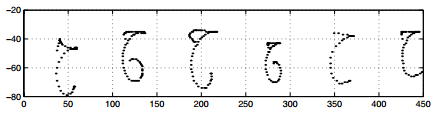
\includegraphics{./figures/ha_different}       
\caption{Different writing styles of the isolated form of the letter \RL{.h}.}
\label{fig:ha_different}
\end{figure}

%%%%%%%%%%%%%%%%%%%%%%%%%%%%%%%%%%%%%%%%%%%%%%
\subsection{Off-line versus On-line Handwriting Recognition}

\iftoggle{edit-mode}{\hspace{0pt}\marginpar{Introduction}}{}
The field of HWR can be classified in several ways. However, the most common categorization is the one that distinguishes between \emph{off-line} (also called static) and \emph{on-line} (also called dynamic).
Off-line HWR focuses on documents that have been written on paper at some previous point of time. A digital image of the document is fed to the computer, and the system attempts to convert the spatial representation of the letters into digital symbols \cite{al2011online}. 
In contrast, on-line HWR is performed on a digital representation of the text written on a special digitizer, tablet or smart-phone device, where sensors pick up the pen-tip movements and the two-dimensional coordinates of successive points of the writing as a function of time are stored.
Figure \ref{fig:offline_vs_online} shows typical input signals that can be analyzed in both cases.

\begin{figure}
	\centering
        \subfloat[]{
            \label{fig:offline}
            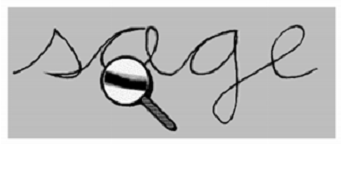
\includegraphics[width=0.5\textwidth]{./figures/offline}
        }
        \subfloat[]{
           \label{fig:online}
           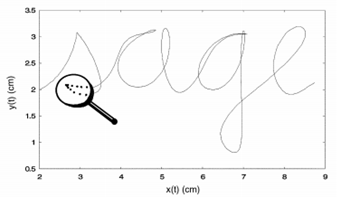
\includegraphics[width=0.5\textwidth]{./figures/online}
        }        
    \caption{An on-line vs. an off-line representation of a word \cite{plamondon2000online}.}
   \label{fig:offline_vs_online}
\end{figure}

\iftoggle{edit-mode}{\hspace{0pt}\marginpar{Similarities and advantages of on-line and off-line}}{}
Off-line HWR techniques can be applied to on-line data by constructing a static image of the on-line script. 
However, it has been shown that the information of the pen dynamics, such as the strokes breaking (i.e., "pen-down" and "pen-up" events) and the order of writing, can be used to obtain a better recognition accuracies than the static data alone. 
In the other direction, the success of on-line systems makes it attractive to consider developing off-line systems that first estimate the trajectory of the writing from the off-line data and then use on-line HWR techniques. 
Nevertheless, reconstructing the temporal data is problematic, and thus, has led to few such systems so far \cite{plamondon2000online}.

\iftoggle{edit-mode}{\hspace{0pt}\marginpar{off-line objectives}}{}
In general, off-line HWR systems are less accurate than on-line systems, but, they are now good enough that they have a significant economic impact on specialized domains such as interpreting handwritten postal addresses on envelopes and reading courtesy amounts on bank checks \cite{melin2007analysis}.

\iftoggle{edit-mode}{\hspace{0pt}\marginpar{A general flow for HWR}}{}
Despite the large variation among the different methods for HWR, there are several fundamental stages that are common between most of the systems.
The data acquisition step is the first stage in HWR. 
In the on-line case, the stylus motion is sampled at equal time intervals.
The samples go through a preprocessing stage that includes filtering of noises, re-sampling the stroke information to obtain equidistant stroke, and normalized to a standard size. 
Additional preprocessing may include slant and slope corrections. 
Then, depending on the nature of the system, the script may undergo segmentation into basic units that could be words, parts of words, single characters or graphemes.
Typically, a feature extraction technique is then applied to extract significant and distinguishing attributes of the input data.
Using a classification algorithm the basic units are labeled. 
In many cases, a post-processing stage is applied in which the language model is used to search for the most likely string in the lexicon.

\iftoggle{edit-mode}{\hspace{0pt}\marginpar{off-line HWR additional steps}}{}
Approaches for on-line and off-line handwriting recognition, while having much in common, are different, due to the disparity in the input data representation. 
Their different nature imposes different challenges and thus variable levels of efforts are required to be spent on the various stages.
The off-line HWR systems usually consist of additional steps of layout analysis and text lines extraction, which are activated at the beginning of the preprocessing stage. 
Each text line is then divided into words or WPs. 
The segmentation, in such system, is made into images that contain basic units. 
The whole process is straightforward for well printed or well written documents; however, in the case of historical or badly printed document much effort is invested in a preprocessing stage that include smoothing, writing flow reconstruction, purification, and more \cite{saba2010survey}. 

%%%%%%%%%%%%%%%%%%%%%%%%%%%%%%%%%%%%%%%%%%%%%%

\subsection{The Holistic versus the Analytic Approach}

\iftoggle{edit-mode}{\hspace{0pt}\marginpar{Importance of the dictionary size}}{}
The vocabulary, from which the words in the test set are taken, has a major impact on how difficult the HWR task is.

\iftoggle{edit-mode}{\hspace{0pt}\marginpar{Closed and open vocabulary definitions}}{}
Closed-vocabulary HWR systems are capable of recognizing words from a predetermined limited size dictionary. 
The restricted vocabulary set is usually called a lexicon.
There are no well-established criteria for the categorization of lexicon size. 
However, the following terms are usually used:
\begin{compactitem}
\item small lexicon - tens of words.
\item medium lexicon - hundreds of words.
\item large lexicon - thousands of words.
\item very large lexicon - tens of thousands of words.
\end{compactitem}
Open-vocabulary tasks refer to the recognition of any word without the constraint of being in a dictionary.

\iftoggle{edit-mode}{\hspace{0pt}\marginpar{Recognition difficulty}}{}
The lexicon is a key-point post-processing stage in many systems, because the linguistic knowledge helps to filter out many possible options that are not included in the lexicon, and consequently raises the recognition rate.
The adhesion to a limited dictionary, may also limit the computational complexity. 
Although most research efforts have been devoted to closed vocabulary systems, open vocabulary systems have also been proposed.
Yet, their accuracy is still far below those relying on a small vocabulary \cite{koerich2003large, shu1996line}.

\iftoggle{edit-mode}{\hspace{0pt}\marginpar{problems imposed by the open vocabulary}}{}
While there exists a wide variety of approaches to cursive script recognition, research in this field has established two main approaches, one is the analytic approach \cite{abdulla2008off, sari2002off, dinges2011offine, elanwar2012unconstrained}, and the other is the holistic approach \cite{biadsy2011segmentation}. 

\iftoggle{edit-mode}{\hspace{0pt}\marginpar{The analytic approach}}{}
The analytic approach involves segmentation of the input curve into basic units and the classification of each individual unit.
The advantage of this approach is that it requires to maintain only a small set of trained models - one for each letter shape - to handle large vocabulary. 
However, the absence of consistent baselines, large variations in writing styles, and seamless connection between letters (connection is done with almost no ligatures) makes segmentation into individual letters very challenging \cite{saabni2009hierarchical}.

\iftoggle{edit-mode}{\hspace{0pt}\marginpar{The holistic approach}}{}
The holistic approach considers the global properties of the written text and recognizes the input word shape as a whole. 
Most popular methods among this group are based on analysis of the number and order of ascenders, descenders, loops and vertical strokes; they often rely on heavy dictionary searching that is costly and prone to be mislead by spelling errors \cite{brodowska2011oversegmentation}.
While it avoids the error-prone segmentation process, in the holistic approach, the recognition system needs to be trained over all words in the dictionary and to maintain and train models for each word. 
Using the holistic approach may be possible for a small vocabulary of words, however, this is not feasible for large vocabularies (20,000 words or more). 
Since each word is constructed from a subset of the character alphabet, it is much more efficient to classify words using the analytic approach \cite{elanwar2012unconstrained}.
In addition, a survey done in \cite{al2011online} on Arabic HWR found that the analytic approach, in general, achieve higher recognition rates than the holistic systems, in cases where words are written in cursive manner, such in the Arabic script. 
This may lead us to conclude that segmentation is a crucial step and that the main problem recognizing Arabic text, especially its handwriting, is its cursiveness.

%%%%%%%%%%%%%%%%%%%%%%%%%%%%%%%%%%%%%%%%%%%%%%%%%%%%%%%

\subsection{Arabic Handwriting Recognition}

\iftoggle{edit-mode}{\hspace{0pt}\marginpar{The Arabic spread}}{}
The Arabic script is one of the descendants of the Aramaic script. 
The earliest known document written using the Arabic script dates from 512 AD.  
The Arabic language is spoken, as their first language, by nearly 350 million people around the world , and written by more than 100 million people, in over 20 different countries \cite{zeki2011segmentation}.
This makes it one of the five most common languages in the world and one of the six United Nations official languages since 1974 \cite{burrow2004arabic}. 
Although Arabic is used mainly in the Arab countries, which consists of about 5.5\% of the world population, almost all Muslims, around 25\% of the world population can read Arabic script as it is the language of the Holy Qur'an \cite{zeki2011segmentation}.

\iftoggle{edit-mode}{\hspace{0pt}\marginpar{The Arabic Alphabet usage in other languages}}{}
The use of Arabic language extended in the 7th and 8th centuries from India to the Atlantic ocean due to the Islamic conquests \cite{saabni2009efficient}. 
Consequently, more than twenty different languages adopted the Arabic alphabet with some changes. 
Examples of such languages are Farsi, Urdu, Malay, Housa and Ottoman Turkish.
Nevertheless, some of those languages has later adopted the Latin characters, but in general, people can still read the Arabic script \cite{zeki2011segmentation}.

\iftoggle{edit-mode}{\hspace{0pt}\marginpar{Literary vs. daily language}}{}
Although spoken Arabic is different from country to country, written Arabic is a standard system used all over the Arab world.
The literary language is called \emph{modern standard Arabic} or \emph{literary Arabic}, which it is currently the only official form of Arabic, used in most written documents as well as in formal spoken occasions, such as lectures and news broadcasts. 

\iftoggle{edit-mode}{\hspace{0pt}\marginpar{The growing interest in the Arabic HWR}}{}
Despite the fact that Arabic alphabets are used in many languages, Arabic Character Recognition has not received sufficient interest from researchers, and therefore, relatively little research progress has been achieved as compared to the progress on Latin or Chinese. 
The first work on Arabic character recognition is by Nazif \cite{nazif1975system} published in 1975, while the earlier research efforts in Latin may be traced back to the middle of the 1940s.
However, considerable increase in the number of research papers related to Arabic character recognition is evident in recent years.
The challenging nature of handwriting recognition and segmentation has attracted the attention of researchers from industry and academic circles \cite{al2010development}.
Despite the growing interest, the challenging problems of Arabic handwriting recognition and segmentation, in both on-line and off-line forms, remain open \cite{zeki2011segmentation}.

%%%%%%%%%%%%%%%%%%%%%%%%%%%%%%%%%%%%%%%%%%%%%%%%%%%%%%%

\subsubsection{Characteristic of the Arabic Writing System}
\label{subsubsec:arabic_writing_characteristic}

\nomenclature{$WP$}{Word part}
\iftoggle{edit-mode}{\hspace{0pt}\marginpar{Basic properties}}{}
The Arabic script consists of 28 basic letters and is written from right to left in a semi-cursive manner in both printed and handwritten forms.
Most letters are written in four different letter shapes depending on their position in the word, e.g., the letter \RL{`}  (Ain) appears as \RL{`}  in its isolated form, \RL{`-} in its initial form, \RL{-`-} in its medial form and \RL{-`} in it final form. 
Among the basic letters, six are Dis-connective - \RL{A} /a/, \RL{d} /d/, \RL{_d} /th/, \RL{r} /r/  \RL{z} /z/ and \RL{w} /w/. 
Dis-connective letters do not connect to the following letter and have only two shapes each, isolated and final. 
The presence of these letters interrupts the continuity of the graphic form of a word. 
The parts of the word that are graphically connected are called \emph{word parts} (WPs). 
If the WP is composed of only one letter, this letter will be in its isolated shape \cite{biadsy2011segmentation}. 

\iftoggle{edit-mode}{\hspace{0pt}\marginpar{Delayed strokes}}{}
Certain characteristics relating to the obligatory dots and strokes of the Arabic script, distinguish it from Latin script.
These dots and strokes are called \emph{delayed strokes} since they are usually drawn last in the when scribing a WP or a word. 
There are mainly two types of delayed strokes, \emph{i'jam} (\RL{A`jAm}) and \emph{harakat} (\RL{.hrkAt}). 
The old Arabic was written without dots or diacritics. 
These additional strokes that were added to the Armaic letters, were first introduced around the 7th century, to prevent the Qur'an from being misread by Muslims \cite{burrow2004arabic}.

\iftoggle{edit-mode}{\hspace{0pt}\marginpar{I'jam}}{}
The i'jam are the pointing diacritics added to the main body of the letter (called rasm) and their role is to distinguish between various constants ,such as, the medial form letters \RL{-b-} /b/, \RL{-t-} /t/, \RL{-_t-} /s/, \RL{-n-} /n/, \RL{-y-} /y/.
Typically, i'jam are not considered diacritics but part of the letter and consists of one or more dots and lines added above, under or inside the letter.
Eliminating, adding or moving a i'jam produces a completely different letter and as a result a completely different word, thus, they are not omitted in the written documents.
Not only dots are used as i'jam, the \RL{'} (hamza) is another type of i'jam that distinguish between the letters \RL{k} /k/ and \RL{l} /l/ in their isolated and final forms.

\iftoggle{edit-mode}{\hspace{0pt}\marginpar{Harakat}}{}
The harakat are small markings added above or below the letters, are used to specify the exact pronunciation of the word.
These diacritics are used in the holy book Qur'an and are commonly used in teaching material and poetry but are seldom used in day-to-day communication and handwriting neither are much in use in the scientific, and business communication.

An example of a fully vocalised Arabic from the Qur'an (Al-Fatiha 1:1):

\begin{center}
\fullvocalize
\transtrue
\begin{RLtext}
bismi al-ll_ahi al-rra.hm_ani al-rra.hImi
\end{RLtext}
In the Name of All'ah, the Most Gracious, the Most Merciful...
\end{center}

\iftoggle{edit-mode}{\hspace{0pt}\marginpar{additional stroke}}{}  
In our work we recognize and classify the main body of the letter and ignore the additional stroke entirely. 
As a result, the number of different letters drops from 29 to 18.
It is important to note that taking the delayed strokes into consideration may be exploited to boost the classification rate.

\iftoggle{edit-mode}{\hspace{0pt}\marginpar{WP count}}{}    
Saabni and El-sana \cite{saabni2009efficient} have explored a large collection of Arabic texts and extracted 300,000 different word combinations of 82,000 different WPs.
Ignoring the delayed strokes, the number of different WP had reduced to 40,000. 

%\iftoggle{edit-mode}{\hspace{0pt}\marginpar{Challenges of the Arabic language}}{}  
%The main body of most Arabic letters is written by a single stroke. A single stroke can contain a single or multiple letters.
%However, there are some letters that usually written using two strokes, such as the letter \RL{-k-}  which is the middle form of the letter \RL{k} /k/. 
%The writer usually writes \RL{-l-} and adds the final upper slanted line when the main body is completed, as if he writes an additional stroke.
%Another problem arises when trying to recognize Arabic transcript, is that, different writers may write the main body of the same word part in a different number of strokes. 
%As can be seen very similar to the \RL{s} /s/ letter in its medial position \RL{-s-}, the only to distinguish between the two options is by looking at the additional strokes.
%For these mentioned complexities, when recognizing Arabic scripts, many researches have preferred the holistic approach. 
%%%%%%%%%%%%%%%%%%%%%%%%%%%%%%%%%%%%%%%%%%%%%%%%%%%%%%%

\subsection{Arabic Script Segmentation}

\iftoggle{edit-mode}{\hspace{0pt}\marginpar{Introduction}}{}
An integral part of the handwriting recognition process, when the analytic approach is considered, is segmentation. 
Therefore, it has long been a critical area of the OCR process. 
As for many pattern recognition problems, the task of segmentation, while usually trivial to a human to perform, is a very challenging pattern recognition problem.
Segmentation and recognition of cursive text are two tasks intertwined and dependent on each other. 
It is believed that wrong segmentation will often results in major contribution to the error of the recognition algorithm \cite{brodowska2011oversegmentation}. 
But, in order to determine the segmentation, the system may try to seek a pattern that will match a member of the system's alphabet \cite{casey1996survey}.
The segmentation task of cursive and unconstrained nature of languages such as Arabic, makes the segmentation task even harder.  
Several segmentation approaches have been proposed in the literature for Arabic OCR, yet, correct and efficient segmentation of the Arabic text is not easily achievable and considered to be a challenging problem even for printed text. 

\iftoggle{edit-mode}{\hspace{0pt}\marginpar{The context dependent of segmentation}}{}
Reliable recognition system requires more than a good matching to a set of letters symbol classes.
The segmentation decision is not a local decision and may affect subsequent segmentation decisions, thus, a poor match of the current segment to some class in the letter library can cast doubt on the correctness of the future segmentation decisions.
In addition, even a series of satisfactory pattern matches can be judged incorrect if contextual requirements of the system output are not satisfied \cite{casey1996survey}.
For instance, in handwritten English, the letter combination "cl" is graphically similar to the letter "d", but in some cases contextually not valid.
In Arabic, two or three consequent appearances of rasm \RL{-b-} /b/ (that is common for the letters \RL{-y-} /y/, \RL{-t-} /t/ and more, see Section \ref{subsubsec:arabic_writing_characteristic}) are very similar to the \RL{-s-} /s/ letter. 
The only way to distinguish between the two options is by considering the delayed strokes and the contextual validity.

\iftoggle{edit-mode}{\hspace{0pt}\marginpar{Approaches for segmentation}}{}
In a comprehensive survey done in \cite{casey1996survey}, the authors has pinpointed two elemental strategies for off-line cursive text segmentation in addition to many approaches that are combinations of these three. 
They have noted that much of the literature on segmentation reports methods that can be characterized as a blend of these three mentioned methods.

\iftoggle{edit-mode}{\hspace{0pt}\marginpar{Dissection}}{}
The first strategy is the classical approach, which is usually named \emph{dissection}, attempts are made to segment the text into primitives. 
Dissection techniques attempt to find appropriate candidate points by learning the characteristic of the segmentation point or by using a rules-based engine. 
Segments, that result from the segmentation process, do not necessarily correspond to exactly one character. 
The word could be segmented into components called graphemes, which are a combination of two or three letters, or a part of a letter. 
The relationship between graphemes and letters is applied in a later phase. 
Many morphological properties were exploited for this task, such as, height, width, separation from neighboring components, low slope if the candidate point local environment, etc.
Various strategies such as projection profile, bounding box or contour tracing exhibit promising results. 
Different types of scripts with essential distinctive nature usually require using different type of properties.
For instance, local minima in the upper or lower contour is commonly used for segmenting English cursive script but not in the Arabic script. 
Such approaches can segment typical words accurately, but, might lead to incorrect segmentation when deal with unconstrained cursive handwriting \cite{saba2010survey}.
A common approach that is followed by many researchers is first over-segmenting of the text, i.e, finding some set of potential splitting points that partition the handwritten word into primitives and then be processed further to eliminate improper candidates point \cite{daifallah2009recognition}.

\iftoggle{edit-mode}{\hspace{0pt}\marginpar{Recognition-based segmentation}}{}
The second approach is the recognition-based segmentation, in which the system searches for sub-components in the cursive text that match letters in its alphabet. 
As mentioned before, character segmentation and character classification are not totally separate steps with a varying degree of dependency.
The initial selection of points can be made in a variety of methods. 
For example, using a moving window with a predefined width which breaks the word into many overlapping pieces without regard to its content.
Then, an iterative or parallel recognition method is used to search for "satisfactory" classification scoring for joint sub-components usually by generating a lattice of all or many possible combinations of the initial candidates set. 
The final decision is determined by the best path through the lattice. 
While avoiding using complex dissection methods, such techniques rely heavily on the classifier accuracy which heavily affects the overall segmentation accuracy \cite{casey1996survey}.

%%%%%%%%%%%%%%%%%%%%%%%%%%%%%%%%%%%%%%%%%%%%%%%%%%%%%%%
\newpage{}
%%%%%%%%%%%%%%%%%%%%%%%%%%%%%%%%%%%%%%%%%%%%%%%%%%%%%%%

\section{Related Work}
\label{sec:related_work}

\iftoggle{edit-mode}{\hspace{0pt}\marginpar{Recognition techniques that uses embedding}}{}

Randa et al. \cite{elanwar2012unconstrained} proposed a two stage on-line Arabic handwritten text segmentation system based on Hidden Markov Model (HMM). 
In the first stage, SPs were nominated, and then, in a second stage, the nominated points were validated using a rules-based engine. 
The system was tested using a self-collected database named OHASD.

Digness et al. \cite{dinges2011offine} used a segmentation-based recognition approach based on dividing the word into smaller pieces, which were afterwards segmented into candidate letters, and then classified into letter classes, using statistical and structural features. 
The $k$-NN classifier was used to obtain the final recognition.

A segmentation-based recognition method that operates on the stroke level for on-line Arabic handwritten words recognition was proposed by Daifallah et al. \cite{daifallah2009recognition}. 
SPs were nominated and then selected by locating semi-horizontal lines moving from right to left. 
A portion of the SPs is filtered out by applying a certain set of rules. 
Then, HMM is used to classify the sub-strokes to letters using the Hu feature. 
The letters candidates and their scoring were used to determine the best set of SPs.\\

%%%%%%%%%%%%%%%%%%%%%%%%%%%%%%%%%%%%%%%%%%%%%%%%%%%%%%%
\newpage{}
%%%%%%%%%%%%%%%%%%%%%%%%%%%%%%%%%%%%%%%%%%%%%%%%%%%%%%%

\section{Scope and Overview}

\iftoggle{edit-mode}{\hspace{0pt}\marginpar{Scope}}{}
The cursiveness of the Arabic script, prima facie, requires delaying the launch of the recognition process until the completion of the word scribing. 
However, in this study, we question the necessity of the requirement by demonstrating the feasibility of approximating the position of the segmentation points (SPs) while the stroke is being written; and by doing so, accelerating the recognition process. 
Furthermore, the obtained information can be used to significantly reduce the potential dictionary size and facilitate a later holistic recognition process.
The proposed method is an analytic approach for handwriting recognition, i.e., it involves segmentation and classification of each part of the text. 
The system operate on the stroke level enabling analysis task related to segmentation and recognition of the stroke into letters to be done while the stroke is being written.

\iftoggle{edit-mode}{\hspace{0pt}\marginpar{Goal}}{}
The emphasis was on finding workable segmentation technique, rather than on the recognition rate.

\iftoggle{edit-mode}{\hspace{0pt}\marginpar{Overview of the system}}{}
The system consists of two main module, one that handles the segmentation and the other handles recognition. 

\iftoggle{edit-mode}{\hspace{0pt}\marginpar{Overview of the system}}{}
The main contributions of the thesis are as follows:
1. create a letters database from the ADAB Database
2. propose a fast trajectory recognition systems
3. propose an an ongoing recognition technique

%The system general flow is seen below:
%\begin{figure}
%\centering
%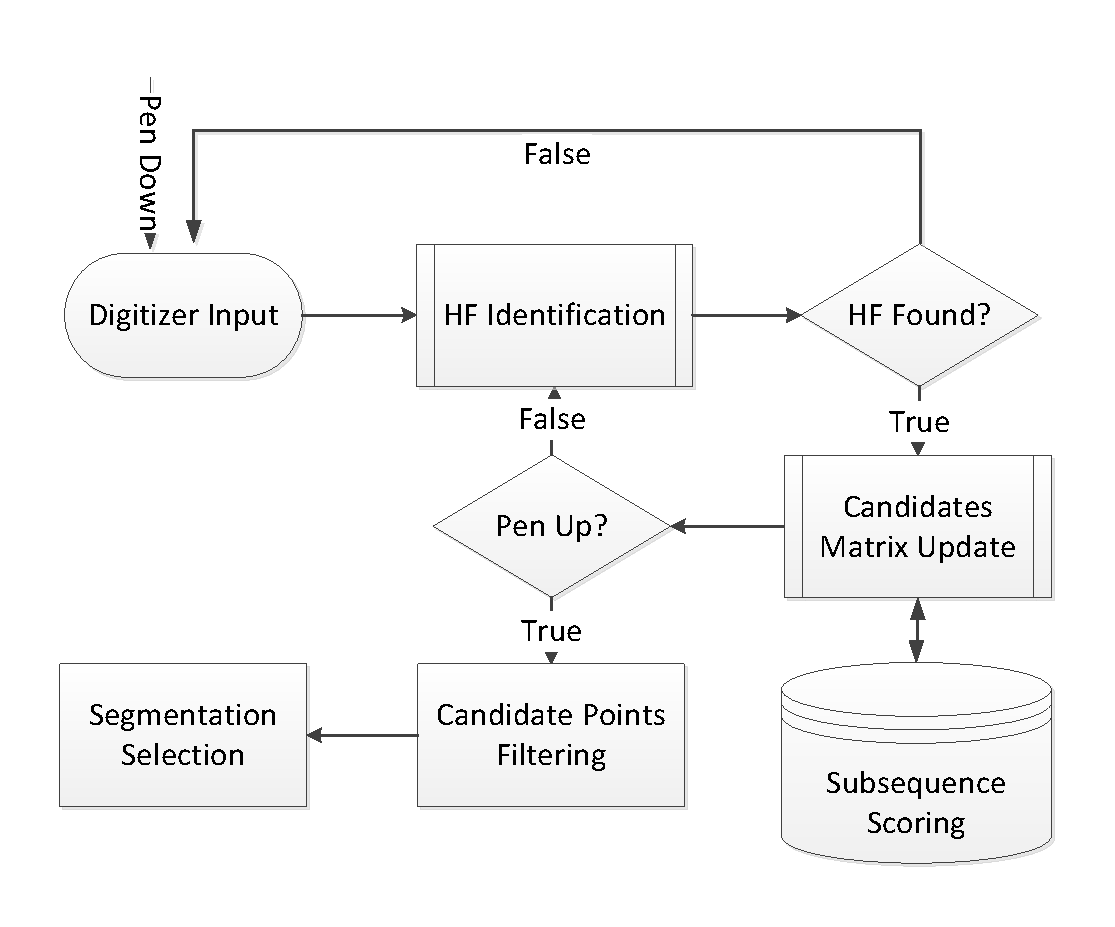
\includegraphics[width=0.8\textwidth]{./figures/system_flow}
%\caption{High level visualization of the system flow.}
%\label{fig:system_flow}
%\end{figure}

%%%%%%%%%%%%%%%%%%%%%%%%%%%%%%%%%%%%%%%%%%%%%%%%%%%%%%%
\newpage{}
%%%%%%%%%%%%%%%%%%%%%%%%%%%%%%%%%%%%%%%%%%%%%%%%%%%%%%%

\section{Thesis Outline}
The organization of the thesis is as follows. 
Chapter \ref{chap:samples_collection} presents the letters extraction process performed on the ADAB database in order to obtain letters samples.

A novel method for Arabic letters classifier is discussed in Chapter \ref{chap:classification}. 
The nearest neighbors classification method is proposed and high performance of the proposed system facilitates it to be used ongoing while the script is being written. The method include a pre-reprocessing task; different feature extraction techniques are discussed; and an embedding to the wavelet domain is exploited in order to renable fast classification using nearest neighbours classification. 

Chapter \ref{chap:segmentation} shows how is the stroke are segmentation point is nominated while the stroke is being scribed, and describe several algorithms for selecting the final segmentation is selected. 

Finally, a summary and future work are proposed in Chapter \ref{conclusions}. 

%\bibliographystyle{plainnat}
%\bibliography{references}
%\end{document}

%TODOs:
%----------
%\begin{enumerate}
%\item See the section "Overview of Arabic Letters" in \cite{abandah2009analysis}. It talks about letters frequencies and special 
%\item Talk about the WP and give statistics of WP length as described in {abandah2009analysis}
%\item Add a table containing the letters in all positions
%\item See \cite{al2011online}.
%\item See \cite{abandah2009analysis}
%\item Review \cite{bahlmann2005advanced} thesis
%\item TODO:see the in introduction of \cite{abandah2009analysis}
%\item See \cite{lorigo2006offline} - motivation section
%\end{enumerate}


%The full list is given in table \ref{table:same_rasm_letters} 
%
%\begin{table}[h]
%\begin{tabular}{ | c | c |}
%\hline
%Letter Set & Positions of similarity\\
%\hline                 
%  \RL{b}, \RL{t}, \RL{_t} & All Positions\\ 
%  \hline
%  \RL{`}, \RL{.g} & All Positions\\
%  \hline
%  \RL{.h}, \RL{j}, \RL{x} & All Positions\\
%  \hline
%  \RL{f}, \RL{q} & All Positions (very slight differences\\ 
%   					&in Isolated mode, the valley of the letter \RL{q} is deeper)\\
%  \hline
%  \RL{r}, \RL{z} & Isolated\\
%  \hline
%  \RL{h}, \RL{T} & Isolated\\
%  \hline
%\end{tabular}
%\centering
%\label{table:same_rasm_letters} 
%\caption{Arabic letters with the same rasm that are diffrentiated by the I'jam}
%\end{table}